% AutoAnalog-RL Round 0 submission report.
% Build: tectonic report.tex   (or pdflatex/xelatex twice; Overleaf works as-is)
\documentclass[10pt,a4paper]{article}

\usepackage[margin=20mm]{geometry}
\usepackage[T1]{fontenc}
\usepackage[utf8]{inputenc}
\usepackage{lmodern}
\usepackage{microtype}
\usepackage{graphicx}
\usepackage{booktabs}
\usepackage{array}
\usepackage{tabularx}
\usepackage{xcolor}
\usepackage{amsmath}
\usepackage{tikz}
\usetikzlibrary{arrows.meta,positioning,calc}
\usepackage{circuitikz}
\usepackage{listings}
\usepackage{caption}
\usepackage[hidelinks]{hyperref}
\usepackage{enumitem}

\definecolor{navy}{RGB}{22,58,107}
\definecolor{pass}{RGB}{26,127,55}
\definecolor{fail}{RGB}{180,35,24}
\definecolor{codebg}{RGB}{242,244,247}

\graphicspath{{figures/}}
\setlength{\parskip}{4pt}
\setlength{\parindent}{0pt}
\captionsetup{font=small,labelfont=bf,skip=4pt}
\renewcommand{\arraystretch}{1.15}
\newcolumntype{L}{>{\raggedright\arraybackslash}X}
\newcolumntype{R}{>{\raggedleft\arraybackslash}p{1.7cm}}
\newcommand{\ok}{\textcolor{pass}{\textbf{pass}}}
\newcommand{\code}[1]{\texttt{#1}}
\lstset{basicstyle=\ttfamily\scriptsize,backgroundcolor=\color{codebg},frame=single,framerule=0pt,breaklines=true,columns=fullflexible,keepspaces=true,xleftmargin=4pt,xrightmargin=4pt}

\title{\vspace{-8mm}\textbf{AutoAnalog-RL}\\[2pt]\large Automated Sizing of High-Speed Interface Circuits via Reinforcement Learning\\[6pt]\normalsize\textbf{Round 0 Submission Report}\\PCIe Gen 2 (5\,Gbps) CTLE + one-tap DFE receiver equalizer $\cdot$ IHP sg13g2 130\,nm open PDK}
\author{Team: \textbf{TEAMNAME}}
\date{15 September 2026}

\begin{document}
\maketitle
\vspace{-6mm}

\begin{center}
\begin{minipage}{0.92\textwidth}
\hrule\vspace{5pt}
\textbf{Abstract.} AutoAnalog-RL sizes a PCIe Gen 2 receiver equalizer with no human in the loop. A Soft Actor-Critic agent drives ngspice directly: every environment step runs a fail-fast DC operating-point check, an AC gate for peaking, a 5\,Gbps PRBS transient through a lossy channel with eye measurement, and an HD3 linearity gate, over a bounded five-parameter CTLE action space (six with the DFE tap). Training happens on the real IHP sg13g2 PSP103 transistor models, compiled from Verilog-A to OSDI and run eight simulators wide on a laptop. The trained policy reaches a design that passes every measured specification --- peaking, power, post-channel eye height and width, HD3, noise and all 45 process/voltage/temperature corners --- in a median of two to three simulations from a random starting point, where a random search needs about thirteen, CMA-ES about nine, and an AC-only bounded search never reaches the eye specification. A two-stage curriculum makes the same policy corner-robust (24/24 rollouts feasible at random PVT corners), an LLM frontend turns plain-language design feedback into reward weights, and the sized netlist is emitted with every design. Along the way the agent exposed two measurement flaws that the manual flow had lived with; both are fixed and documented here.
\vspace{5pt}\hrule
\end{minipage}
\end{center}

\section{Introduction and objectives}
Sizing analog front-end circuits is a search over a handful of continuous device values against a set of coupled specifications, evaluated by a slow simulator. For a receiver equalizer the coupling is severe: the same transistor width sets gain, bandwidth, power, linearity and noise, and the specification that matters most --- the eye opening after the channel --- is only visible in a transient simulation. Manual sweeps do not scale, and generic optimisers spend most of their simulation budget in infeasible regions.

The Round 0 synopsis proposed AutoAnalog-RL: a sample-efficient Soft Actor-Critic (SAC) agent paired with a headless Python-to-ngspice pipeline over a bounded 5-parameter action space, with fail-fast DC checks, curriculum learning across 45 PVT corners, an LLM frontend that maps natural-language feedback to reward weights, and a production-ready schematic as the output. Table~\ref{tab:synopsis} lists each promise and its status.

\begin{table}[h]\small
\begin{tabularx}{\textwidth}{L L}
\toprule
\textbf{Synopsis promise} & \textbf{Status in this submission}\\
\midrule
PCIe Gen 2 (5\,Gbps) CTLE + 1-tap DFE sized with zero human intervention & \ok. SAC sizes the CTLE end to end; the DFE tap is either swept per design or sized by the agent (\code{--equalizer}). Section~\ref{sec:curriculum}.\\
Skywater 130\,nm PDK & \textcolor{fail}{\textbf{Changed}} to the IHP sg13g2 130\,nm PDK (the brief allows either); reason in Section~\ref{sec:pdk}.\\
Sample-efficient SAC agent & \ok. Converges within $\sim$2k environment steps; median 2--3 simulations to a feasible design. Section~\ref{sec:results}.\\
Headless Python-to-ngspice pipeline & \ok, including a Windows toolchain for the PSP103 OSDI models. Section~\ref{sec:backend}.\\
Bounded 5-parameter action space, fail-fast DC checks & \ok. Section~\ref{sec:rl}.\\
Curriculum learning across 45 PVT corners & \ok. Nominal stage then corner-randomised stage; 24/24 rollouts feasible at random corners. Section~\ref{sec:curriculum}.\\
LLM frontend: natural-language feedback to reward weights & \ok. Section~\ref{sec:llm}.\\
Production-ready schematic, faster than manual sweeps & \ok. Sized netlist per design; 2 vs $\sim$13 simulations; the 100-candidate search fails the eye. Sections~\ref{sec:results} and \ref{sec:deliverables}.\\
\bottomrule
\end{tabularx}
\caption{Synopsis deliverables and their status.}\label{tab:synopsis}
\end{table}

\subsection{Problem-statement compliance}
The Nebula ``AI/ML for Analog Circuit Design'' brief asks for a fully automated RL framework that sizes an equalizer for a PCIe PHY from target specifications with zero human intervention, in significantly less time than sweeping the MOS/R/C/L space, on an open PDK (IHP 130\,nm BiCMOS or SkyWater sky130). Table~\ref{tab:brief} maps each specification in the brief to this submission; ``ours'' is the tighter internal target the RL reward uses, and results are the curriculum policy's best design unless noted.

\begin{table}[h]\small
\begin{tabularx}{\textwidth}{L L L l}
\toprule
\textbf{Brief specification} & \textbf{Ours (reward target)} & \textbf{Result} & \textbf{Status}\\
\midrule
Nyquist 2.5\,GHz (PCIe Gen 2, 5.0\,Gbps) & 2.5\,GHz, 5\,Gbps PRBS7 & measured at 2.5\,GHz & \ok\\
HF peaking boost 3--12\,dB, tunable 1.25--2.5\,GHz & 3--12\,dB at the configured Nyquist frequency & 4.5\,dB at 2.5\,GHz; \code{--spec nyquist\_frequency\_hz=1.25e9} retunes rate, channel and measurement; retuned policy 20/20, 5.23\,dB at 1.25\,GHz (Section~\ref{sec:tunable}) & \ok\\
1-stage CTLE with source degeneration (variable $R_s$, $C_s$) & $R_s$ 10--500\,$\Omega$, $C_s$ 1\,fF--1\,pF in the action & yes & \ok\\
1-tap DFE; NRZ signalling & behavioural one-tap DFE, tap swept or RL-sized; NRZ PRBS7 & tap $+0.062$ opens 0.325\,V to 0.355\,V (equalizer run) & \ok\ (behavioural)\\
HD3 $< -30$\,dB (100\,MHz differential input) & $\le -30$\,dB, enforced in the reward & $-61.9$\,dB & \ok\\
Input-referred noise $< 1.5$\,mV\,rms (10\,MHz--5\,GHz) & reported & 0.242\,mV\,rms & \ok\\
Power $< 15$\,mW & $\le 2$\,mW & 1.12\,mW & \ok\\
Area $< 0.05$\,mm$^2$ (130\,nm PDK) & reported, first-order & $1.1\times10^{-5}$\,mm$^2$ active-device estimate & \ok\ (estimate)\\
Eye opening $> 0.4$\,UI (H) and $> 100$\,mV (V) & $\ge 0.7$\,UI and $\ge 0.25$\,V after a $-10$\,dB channel & 0.90\,UI, 0.370\,V & \ok\\
PVT: TT/SS/FF/SF/FS, VDD $\pm5\%$, 0--125\,$^\circ$C & the same 45 corners, trained across (curriculum) and verified & 45/45 & \ok\\
Zero human intervention; faster than sweeping & policy sizes from a random start in 2--3 simulations & random search 13, CMA-ES 9 & \ok\\
Deliverable: Python RL framework, specs in, SPICE in the loop, schematic + specs out & \code{train\_sac.py --spec ...}, ngspice gates, \code{sized\_ctle.sp} + \code{validation.json} & yes & \ok\\
Bonus: LLM-based human interaction to fine-tune & \code{reward\_from\_feedback.py} $\rightarrow$ \code{--reward-settings} & yes (applies per run/stage) & \ok\\
\bottomrule
\end{tabularx}
\caption{The brief's specifications against this submission.}\label{tab:brief}
\end{table}

Under the brief's own eye thresholds (100\,mV, 0.4\,UI) the pre-ML AC-only bounded-search design (0.160\,V, 0.58\,UI) also passes; the RL reward uses the tighter 0.25\,V / 0.7\,UI targets so that the policy delivers margin rather than a marginal pass, and the comparisons in this report are against those.

\section{System overview}
Figure~\ref{fig:arch} shows the loop. The agent's action is a normalised design vector; the evaluator maps it to device values, renders the CTLE netlist, and runs the gates in order, stopping at the first failure so that infeasible designs cost as little simulation as possible. Metrics feed a transparent reward; the environment returns the design, its metrics and normalised constraint violations as the observation. Everything after the simulator adapter is simulator-agnostic.

\begin{figure}[h]\centering
\resizebox{\textwidth}{!}{%
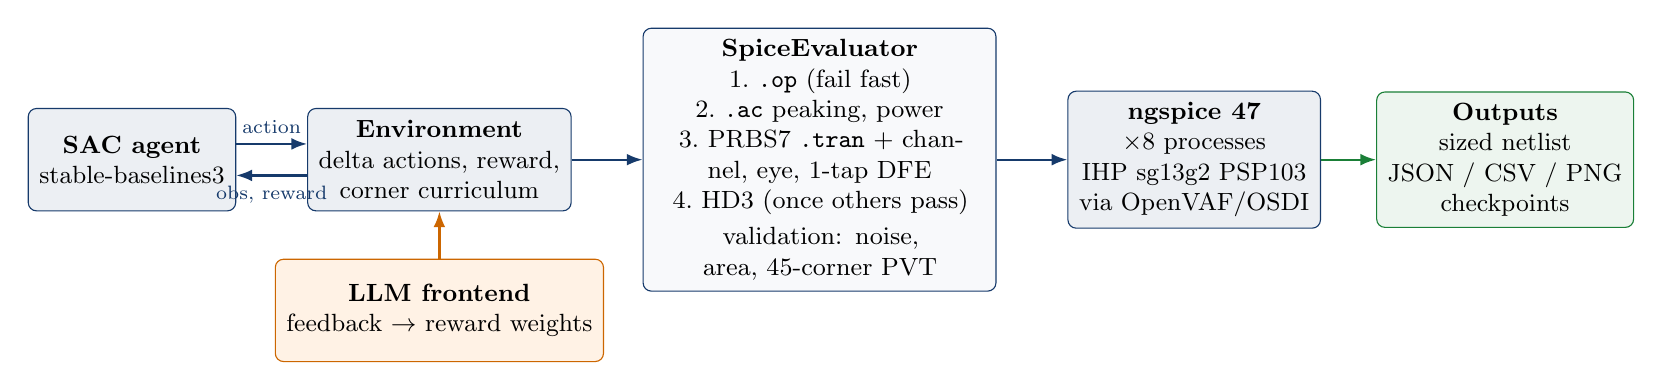
\begin{tikzpicture}[font=\small, box/.style={draw=navy, fill=navy!8, rounded corners=3pt, align=center, minimum height=13mm, inner sep=4pt}, arr/.style={-{Latex[length=2mm]}, navy, thick}]
\node[box] (agent) {\textbf{SAC agent}\\stable-baselines3};
\node[box, right=9mm of agent] (env) {\textbf{Environment}\\delta actions, reward,\\corner curriculum};
\node[box, right=9mm of env, fill=navy!3, text width=42mm] (ev) {\textbf{SpiceEvaluator}\\1.\ \code{.op} (fail fast)\\2.\ \code{.ac} peaking, power\\3.\ PRBS7 \code{.tran} + channel, eye, 1-tap DFE\\4.\ HD3 (once others pass)\\[2pt]validation: noise, area, 45-corner PVT};
\node[box, right=9mm of ev] (ng) {\textbf{ngspice 47}\\$\times$8 processes\\IHP sg13g2 PSP103\\via OpenVAF/OSDI};
\node[box, right=7mm of ng, draw=pass, fill=pass!8] (out) {\textbf{Outputs}\\sized netlist\\JSON / CSV / PNG\\checkpoints};
\node[box, below=6mm of env, draw=orange!80!black, fill=orange!10] (llm) {\textbf{LLM frontend}\\feedback $\rightarrow$ reward weights};
\draw[arr] ([yshift=2mm]agent.east) -- ([yshift=2mm]env.west) node[midway, above, font=\scriptsize]{action};
\draw[arr] ([yshift=-2mm]env.west) -- ([yshift=-2mm]agent.east) node[midway, below, font=\scriptsize]{obs, reward};
\draw[arr] (env) -- (ev);
\draw[arr] (ev) -- (ng);
\draw[arr, pass] (ng) -- (out);
\draw[arr, orange!80!black] (llm) -- (env);
\end{tikzpicture}}
\caption{AutoAnalog-RL loop. The evaluator runs the ngspice gates in fail-fast order; the environment and reward are simulator-agnostic; the LLM frontend adjusts reward weights between runs.}\label{fig:arch}
\end{figure}

The repository (\code{al\_nebula}) is organised by responsibility: \code{netlists/} owns the CTLE topology, \code{spice/} the simulator adapter and every measurement, \code{rl/} the specifications, reward, environment, DFE model, PVT matrix and LLM feedback parser, \code{scripts/} the training, baseline, evaluation, validation and reporting entry points, and \code{tests/} a 59-test regression suite that runs without ngspice.

\section{Process design kit}\label{sec:pdk}
The brief allows either open 130\,nm PDK (IHP BiCMOS or SkyWater sky130); the synopsis named sky130. The implementation targets the IHP sg13g2 open PDK. The team switched during development because the sky130 simulation flow was too slow for an RL loop that runs three ngspice analyses per environment step, whereas IHP's PSP103 Verilog-A models compile with OpenVAF to OSDI and run natively in ngspice 47 at about 0.6\,s per environment step with eight simulators in parallel. PSP103 is a foundry-grade surface-potential compact model, so this is a strengthening of the device physics rather than a simplification. The framework is PDK-agnostic by construction: the generic Level-1 and IHP paths share every line of code except the model library selected by \code{SpiceEvaluator.for\_model\_source()}, so a sky130 backend is a netlist variant plus a corner-library mapping.

\section{Circuit, channel and simulation backend}\label{sec:backend}
\subsection{Circuit and specifications}
The CTLE is a differential NMOS pair with resistive loads and RC source degeneration (Figure~\ref{fig:ctle}). The agent sizes five values: input width $W_\mathrm{in}$, load $R_\mathrm{load}$, tail current $I_\mathrm{bias}$, degeneration resistance $R_s$ and degeneration capacitance $C_s$ (Table~\ref{tab:bounds}). The transient gate drives a two-period PRBS7 at 5\,Gbps through a two-section RC channel with about $-10$\,dB loss at the 2.5\,GHz Nyquist frequency (the loss slope of a PCIe Gen 2 class FR-4 trace); the DC and AC gates bypass the channel so peaking measures the CTLE alone. A one-tap decision-feedback stage operates on the UI-centre samples of the CTLE output.

\begin{figure}[h]
\begin{minipage}[c]{0.56\textwidth}\centering
\begin{circuitikz}[scale=0.8, transform shape, american]
\draw (0,5) node[left]{VDD (1.2\,V)} -- (6,5);
\draw (1,5) to[R, l_=$R_\mathrm{load}$] (1,3.4) node[circ]{} node[left]{outP};
\draw (5,5) to[R, l=$R_\mathrm{load}$] (5,3.4) node[circ]{} node[right]{outN};
\draw (1,3.4) node[nmos, anchor=D, rotate=0](m1){} (m1.G) node[left]{inP} ;
\draw (5,3.4) node[nmos, anchor=D, xscale=-1](m2){} (m2.G) node[right]{inN};
\node[right=1pt of m1.D, yshift=-4mm, font=\scriptsize]{M1 $W_\mathrm{in}$};
\node[left=1pt of m2.D, yshift=-4mm, font=\scriptsize]{M2 $W_\mathrm{in}$};
\draw (m1.S) to[R, l_=$R_s$] (3,1.3) to[R, l_=$R_s$] (m2.S);
\draw (m1.S) to[C, l=$C_s$] (m2.S);
\draw (3,1.3) to[I, l=$I_\mathrm{bias}$] (3,-0.2) node[ground]{};
\end{circuitikz}
\captionof{figure}{Source-degenerated differential CTLE; the five sized values are labelled. Devices are IHP sg13g2 \code{sg13\_lv\_nmos}, $L=130$\,nm.}\label{fig:ctle}
\end{minipage}\hfill
\begin{minipage}[c]{0.40\textwidth}\small
\begin{tabular}{lrr}
\toprule
\textbf{Parameter} & \textbf{Lower} & \textbf{Upper}\\
\midrule
$W_\mathrm{in}$ & 0.5\,$\mu$m & 50\,$\mu$m\\
$R_\mathrm{load}$ & 100\,$\Omega$ & 1000\,$\Omega$\\
$I_\mathrm{bias}$ & 0.1\,mA & 2\,mA\\
$R_s$ & 10\,$\Omega$ & 500\,$\Omega$\\
$C_s$ & 1\,fF & 1\,pF\\
DFE tap (optional 6th) & $-0.5$ & $+0.5$\\
\bottomrule
\end{tabular}
\captionof{table}{Bounded action space; actions in $[-1,1]$ map linearly onto these ranges.}\label{tab:bounds}
\end{minipage}
\end{figure}

\begin{table}[h]\small
\begin{tabularx}{\textwidth}{L L L L}
\toprule
\textbf{Specification} & \textbf{Target} & \textbf{Gate} & \textbf{In the reward?}\\
\midrule
High-frequency peaking at 2.5\,GHz & 3\,dB $\le$ peaking $\le$ 12\,dB & \code{.ac} 10\,MHz--10\,GHz & yes\\
Power & $\le 2$\,mW & \code{.op} & yes, plus a continuous charge inside the feasible set\\
Eye height after channel & $\ge 0.25$\,V (IHP; 0.5\,V on the Level-1 model) & PRBS7 \code{.tran} & yes\\
Eye width after channel & $\ge 0.7$\,UI & PRBS7 \code{.tran} & yes\\
HD3 at 100\,MHz, 100\,mV$_\mathrm{pp,diff}$ & $\le -30$\,dB & single-tone \code{.tran} & with \code{--hd3}\\
Input-referred noise, 10\,MHz--5\,GHz & $\le 1.5$\,mV\,rms & \code{.noise} & validation only\\
Area & reported & first-order device geometry & validation only\\
PVT & 45/45 corners pass peaking & 5 process $\times$ 3 supply $\times$ 3 temperature & curriculum (Section~\ref{sec:curriculum}) and validation\\
\bottomrule
\end{tabularx}
\caption{Specifications, the gate that measures each, and whether it shapes the reward.}
\end{table}

\subsection{Simulation backend}
The sg13g2 transistor deck uses PSP103, which ngspice loads as OSDI shared libraries compiled from the PDK's Verilog-A sources with OpenVAF-reloaded. The original evidence run used a Linux build; this submission adds a Windows path so training could run on the team's laptop: OpenVAF's Windows binary expects MSVC's \code{link.exe}, and a small drop-in linker shim (\code{tools/openvaf-link-shim}) rewrites its link line for 64-bit MinGW, supplying the \code{\_\_chkstk} stack probe and the UCRT import. The resulting \code{psp103.osdi}, \code{psp103\_nqs.osdi} and \code{mosvar.osdi} load in the stock ngspice 47 Windows build and reproduce the Linux AC and HD3 numbers to every printed digit.

Throughput mattered more than any single simulation: one PSP103 transient takes about 1.5\,s, but eight in parallel initially took 90\,s each, because ngspice ignores \code{OMP\_NUM\_THREADS} and spins its own OpenMP pool per process; with eight processes the spin-waiting threads oversubscribed the twelve cores by an order of magnitude. Pinning each ngspice to one thread through the generated \code{.spiceinit} restored 1.4\,s for eight concurrent transients, a 65$\times$ difference, and is what makes 0.6\,s per environment step possible. The environments run on threads rather than processes because \code{subprocess.run} releases the GIL while ngspice runs, and spawning eight Python workers that each load CUDA torch failed DLL initialisation on Windows.

\section{Reinforcement-learning formulation}\label{sec:rl}
\textbf{State.} The normalised design vector, a DC-valid flag, the four scaled metrics (peaking, power, eye height, eye width) and the normalised violation of every enforced constraint. \textbf{Action.} A delta on the design vector, scaled by 0.2 and clipped to the box, so the agent sizes incrementally; the whole-equalizer variant adds the DFE tap. \textbf{Episode.} Up to 30 steps from a random design; a DC failure is penalised but does not end the episode, so the agent can step back out of an invalid region.

\textbf{Reward.} With normalised violations $v_i$ (1.0 is a full specification's worth of miss) and weights $w_i$:
\begin{align*}
r &= -\sum_i w_i v_i \;-\; w_\mathrm{eff}\min\!\left(1, \tfrac{P}{P_\mathrm{max}}\right) \;+\; [\text{all specs met}]\,\big(B_\mathrm{success} + w_\mathrm{margin}\min(1, \text{tightest margin})\big),\\
r &= -10 \quad\text{on a DC failure.}
\end{align*}
The continuous power charge keeps a gradient inside the feasible set; the success bonus (20) and the margin bonus (weight 5) pull the agent into, not onto, the feasible region. \textbf{Algorithm.} SAC (stable-baselines3 2.9) with automatic entropy tuning from 0.1, batch 256, one gradient step per environment step, 500 random warm-up steps, eight parallel environments.

\subsection{Why the first runs plateaued, and the fix}
The first SAC runs (5000 steps on the generic Level-1 model) reached a feasible design in about 85\% of episodes but never became reliable and did not beat random search. Two causes: the episode ended on the first feasible step, so nothing rewarded margin and the policy sat exactly on the eye-height boundary where action noise pushed it off; and a $-100$ DC penalty dwarfed the unit-scale shaping costs, so the critic spent its capacity on a cliff. Keeping the episode running after success (\code{--hold-on-success}), paying for margin, and a $-10$ DC penalty fixed it: on Level-1 the policy went from 79\% to 95\% feasible steps by 5k steps, with the median eye height moving from 0.43\,V to 0.92\,V against a 0.5\,V spec. Deterministic rollouts of the Level-1 policy reach feasibility in 20/20 cases, median 2.5 steps.

\subsection{Eye-height target on the real models}
The eye targets had been calibrated so that about one in ten random Level-1 designs passes. On PSP103 none of 400 random designs reaches 0.5\,V (best 0.45\,V, median 0.17\,V): the real devices have roughly half the gain. The IHP target is therefore 0.25\,V, which restores the same 10\% random feasibility and sits above the $\sim$175\,mV differential eye PCIe Gen 2 requires at the receiver.

\section{Results on the IHP models}\label{sec:results}
All runs use \code{--model-source ihp --eye-height-min 0.25 --n-envs 8 --hold-on-success --random-reset --margin-weight 5 --invalid-penalty -10 --max-steps 30 --batch-size 256 --gradient-steps -1 --ent-coef auto\_0.1}. ``Training feasible'' is the fraction of environment steps in the last 4k steps at which every enforced specification was met. Evaluation (\code{scripts/evaluate\_policy.py}) rolls the trained policy out deterministically from 20 random starting designs, then validates the best design with the full gate set and all 45 PVT corners.

\begin{table}[h]\scriptsize
\begin{tabularx}{\textwidth}{l r L r r l L}
\toprule
\textbf{Run} & \textbf{Steps} & \textbf{Variant} & \textbf{Train.\ feas.} & \textbf{Rollouts} & \textbf{Steps (med./worst)} & \textbf{Best design: eye, power, HD3, PVT}\\
\midrule
sac-ihp-v1 (seed 1) & 30k & -- & 95.5\% & 20/20 & 2 / 4 & 0.327\,V, 1.22\,mW, $-57.8$\,dB, 45/45\\
sac-ihp-v1-s2 (seed 2) & 12k & -- & 95.5\% & 20/20 & 3 / 4 & 0.316\,V, 1.22\,mW, $-57.7$\,dB, 45/45\\
sac-ihp-v1-s3 (seed 3) & 12k & -- & 95.5\% & 20/20 & 2.5 / 4 & 0.348\,V, 1.33\,mW, $-60.2$\,dB, 45/45\\
sac-ihp-hd3 & 12k & HD3 enforced in the reward & 95.6\% & 20/20 & 2.5 / 4 & 0.335\,V, 1.24\,mW, $-58.1$\,dB, 45/45\\
sac-ihp-pvt (curriculum stage 2) & +8k & resumed from sac-ihp-hd3; random PVT corner per episode; HD3 enforced & 95.4\% & 24/24 at random corners & 2 / 4 & 0.370\,V, 1.12\,mW, $-61.9$\,dB, 45/45\\
sac-ihp-eq (whole equalizer) & 8k & six-value action: CTLE + DFE tap; post-DFE eye drives the reward & 92.3\% & 20/20 & 3 / 5 & 0.325\,V raw, 0.355\,V post-DFE (tap $+0.062$), 1.36\,mW, $-71.6$\,dB, 45/45\\
sac-ihp-gen1 (retune) & +3k & resumed from sac-ihp-v1 with \code{--spec nyquist\_frequency\_hz=1.25e9} (PCIe Gen 1, 2.5\,Gbps) & 96.5\% & 20/20 & 2 / 5 & 5.23\,dB at 1.25\,GHz, 0.350\,V, 1.28\,mW, $-70.9$\,dB, 45/45\\
\bottomrule
\end{tabularx}
\caption{Training runs on the IHP sg13g2 PSP103 models. Every best design passes peaking, power, eye height and width, HD3, noise and all 45 corners.}\label{tab:runs}
\end{table}

Over the three seeds of the base configuration: 60 of 60 rollouts feasible, mean steps to a feasible design $2.53\pm0.06$, best-design eye $0.330\pm0.014$\,V, power $1.26\pm0.05$\,mW, HD3 $-58.6\pm1.2$\,dB, best reward $20.70\pm0.04$ (mean $\pm$ std over seeds).

\begin{figure}[h]\centering
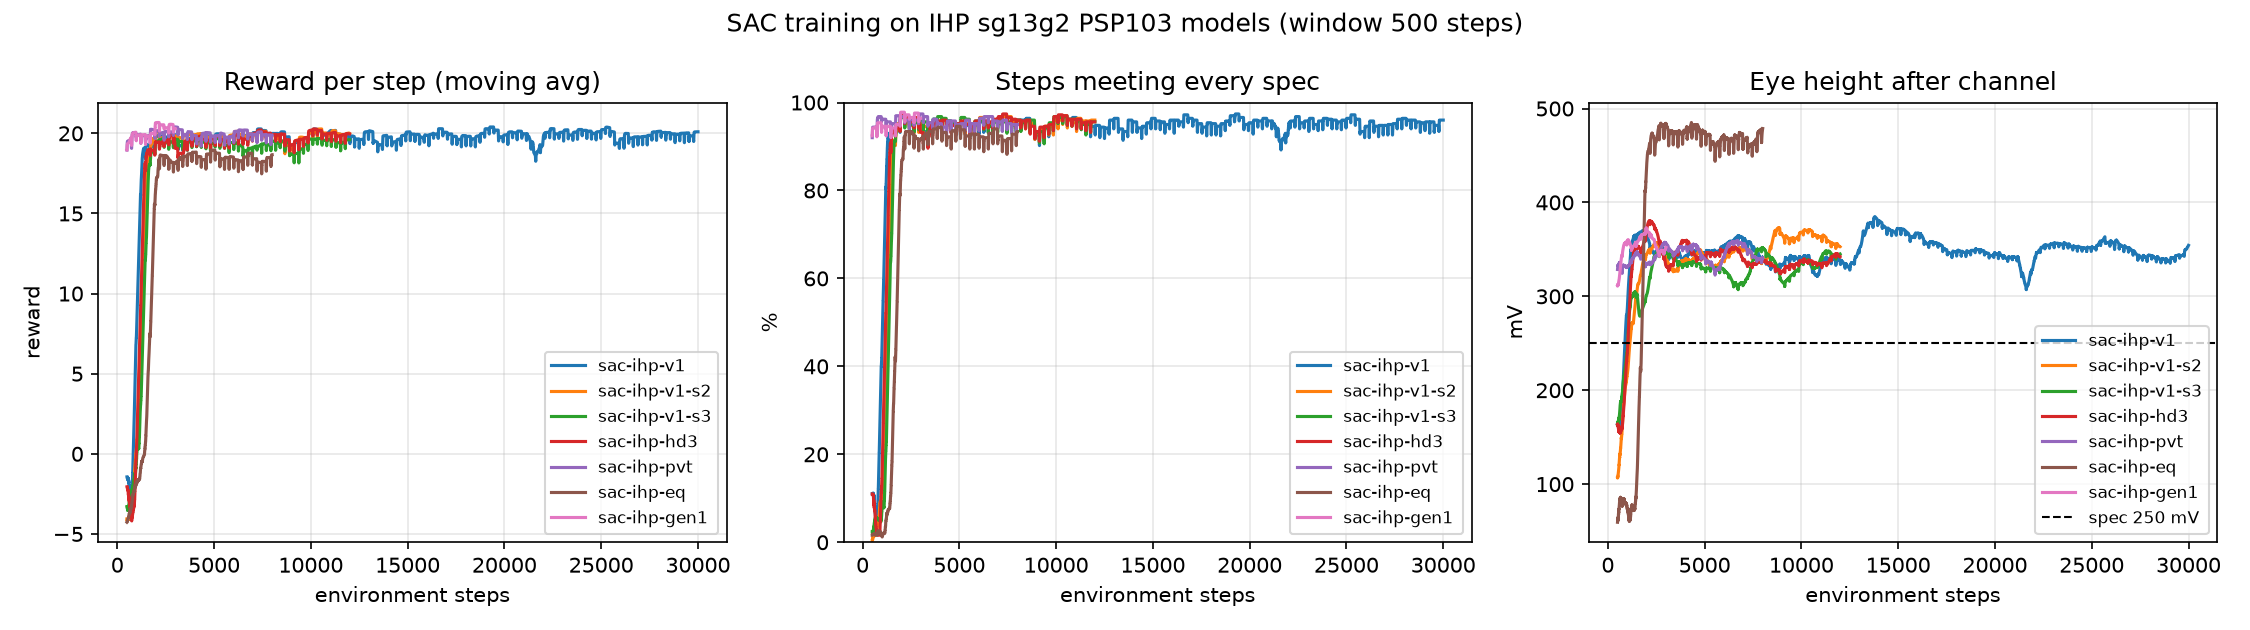
\includegraphics[width=0.98\textwidth]{learning_curves}
\caption{Learning curves for the IHP runs (500-step moving average): reward per step, fraction of steps meeting every specification, and post-channel eye height against the 0.25\,V target. All runs converge within about 2k steps; the curriculum and retune stages start converged because they resume a trained policy.}\label{fig:curves}
\end{figure}

\subsection{Baselines: random search and CMA-ES}
Two baselines run against the same models and reward. Random search (\code{scripts/baseline\_random.py}, 3000 designs): 7.9\% of designs satisfy every specification (238/3000) and the first feasible one is design 27. CMA-ES (\code{scripts/baseline\_cmaes.py}, population 8, $\sigma_0=0.5$ in the normalised box): three 400-evaluation trials from the box centre and six 96-evaluation trials from random starting designs, the latter matching how the policy is rolled out (Table~\ref{tab:baselines}, Figure~\ref{fig:budget}).

\begin{table}[h]\small
\begin{tabularx}{\textwidth}{L r r L}
\toprule
\textbf{Method (from random starting designs unless noted)} & \textbf{First feasible (med./worst)} & \textbf{Best reward at 50 sims} & \textbf{Cost per new instance}\\
\midrule
SAC policy, deterministic rollouts (144 rollouts over 7 evaluations) & \textbf{2--3 / 5} & 20.5--20.8 & 2--3 simulations, no search\\
CMA-ES, random start (6 trials) & 9 / 24 & 20.50 (mean) & $\sim$10 simulations to feasible; 400 to refine\\
CMA-ES from the box centre (3 trials) & 2--5 & 20.8--21.1; 21.3--21.4 at 400 & 400 simulations per design\\
Random search & 27 & 19.65 & $\sim$13 simulations per feasible design\\
\bottomrule
\end{tabularx}
\caption{Simulation cost to a feasible design and reward at equal budget, policy versus baselines.}\label{tab:baselines}
\end{table}

CMA-ES is a strong per-instance optimiser on this five-dimensional problem: given 400 simulations it reaches the same reward the policies reach during training (21.2--21.6), and from the fortuitously near-feasible box centre it finds a feasible design in a handful of evaluations. The policy's advantage is amortisation and robustness: after one training run it sizes a new instance --- a random starting design, a random PVT corner, a re-weighted reward --- in two to three simulations with no per-instance search, three to four times fewer than CMA-ES from the same starts and about ten times fewer than random sampling. Refinement inside the feasible set is what the hold-on-success training phase does; the rollouts reported here stop at the first feasible step. The AC-only 100-candidate bounded search of the pre-ML pipeline, which selects on peaking alone, produces a design with a post-channel eye of only 0.160\,V.

\begin{figure}[h]\centering
\begin{minipage}[t]{0.49\textwidth}\centering
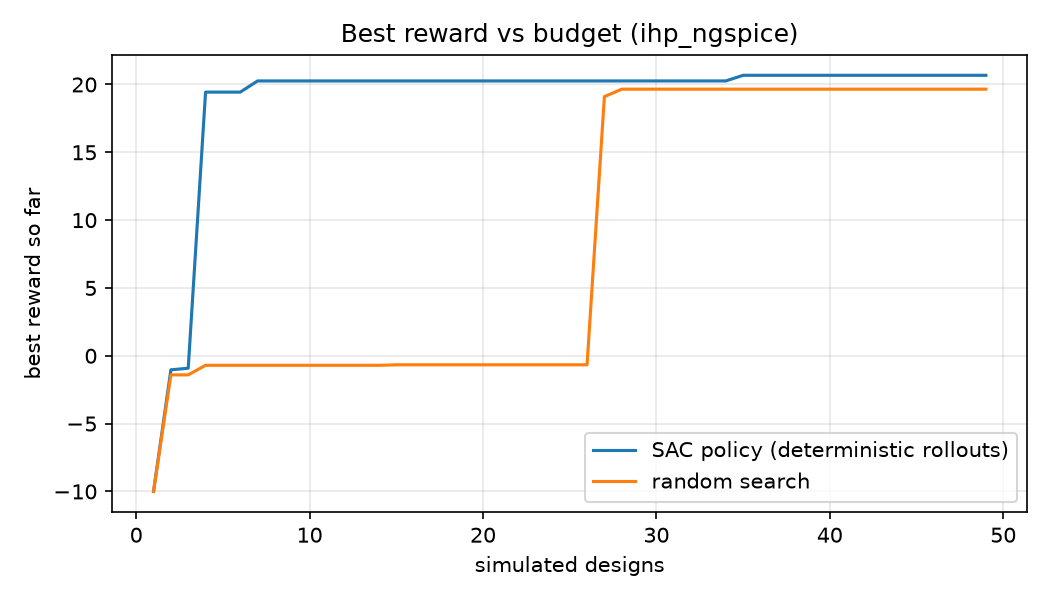
\includegraphics[width=\textwidth]{budget_curve}
\caption{Best reward found versus number of simulated designs, policy rollouts against random search (seed 1).}\label{fig:budget}
\end{minipage}\hfill
\begin{minipage}[t]{0.49\textwidth}\centering
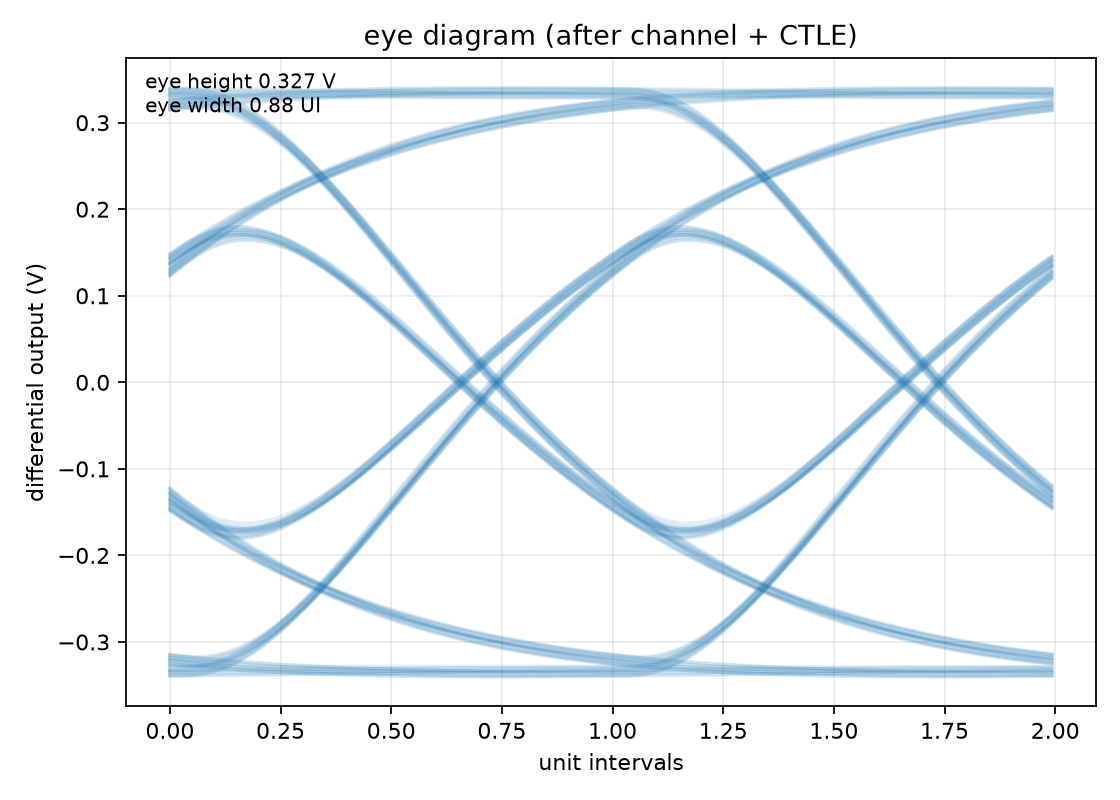
\includegraphics[width=\textwidth]{eye_diagram}
\caption{Two-UI eye diagram of the seed-1 policy design after the $-10$\,dB channel: 0.327\,V / 0.88\,UI.}
\end{minipage}
\end{figure}
\begin{figure}[h]\centering
\begin{minipage}[t]{0.49\textwidth}\centering
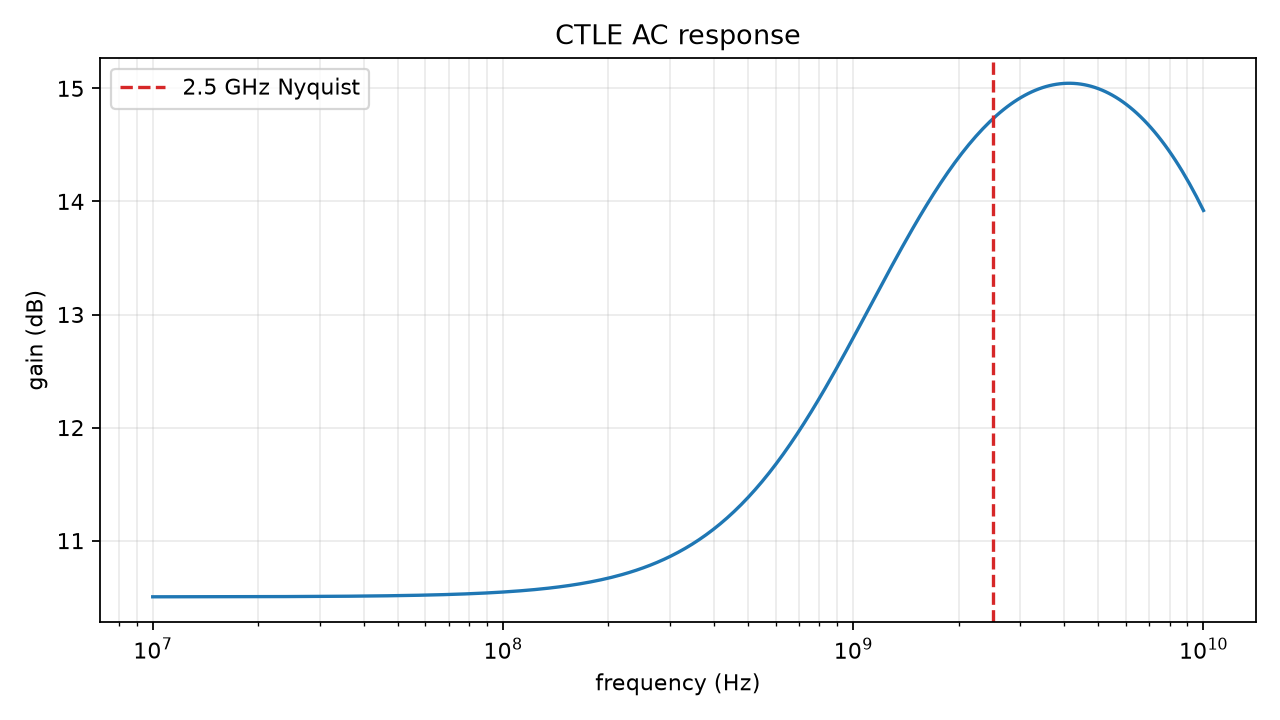
\includegraphics[width=\textwidth]{ac_response}
\caption{AC response of the same design: 4.2\,dB of peaking at the 2.5\,GHz Nyquist frequency.}
\end{minipage}\hfill
\begin{minipage}[t]{0.49\textwidth}\centering
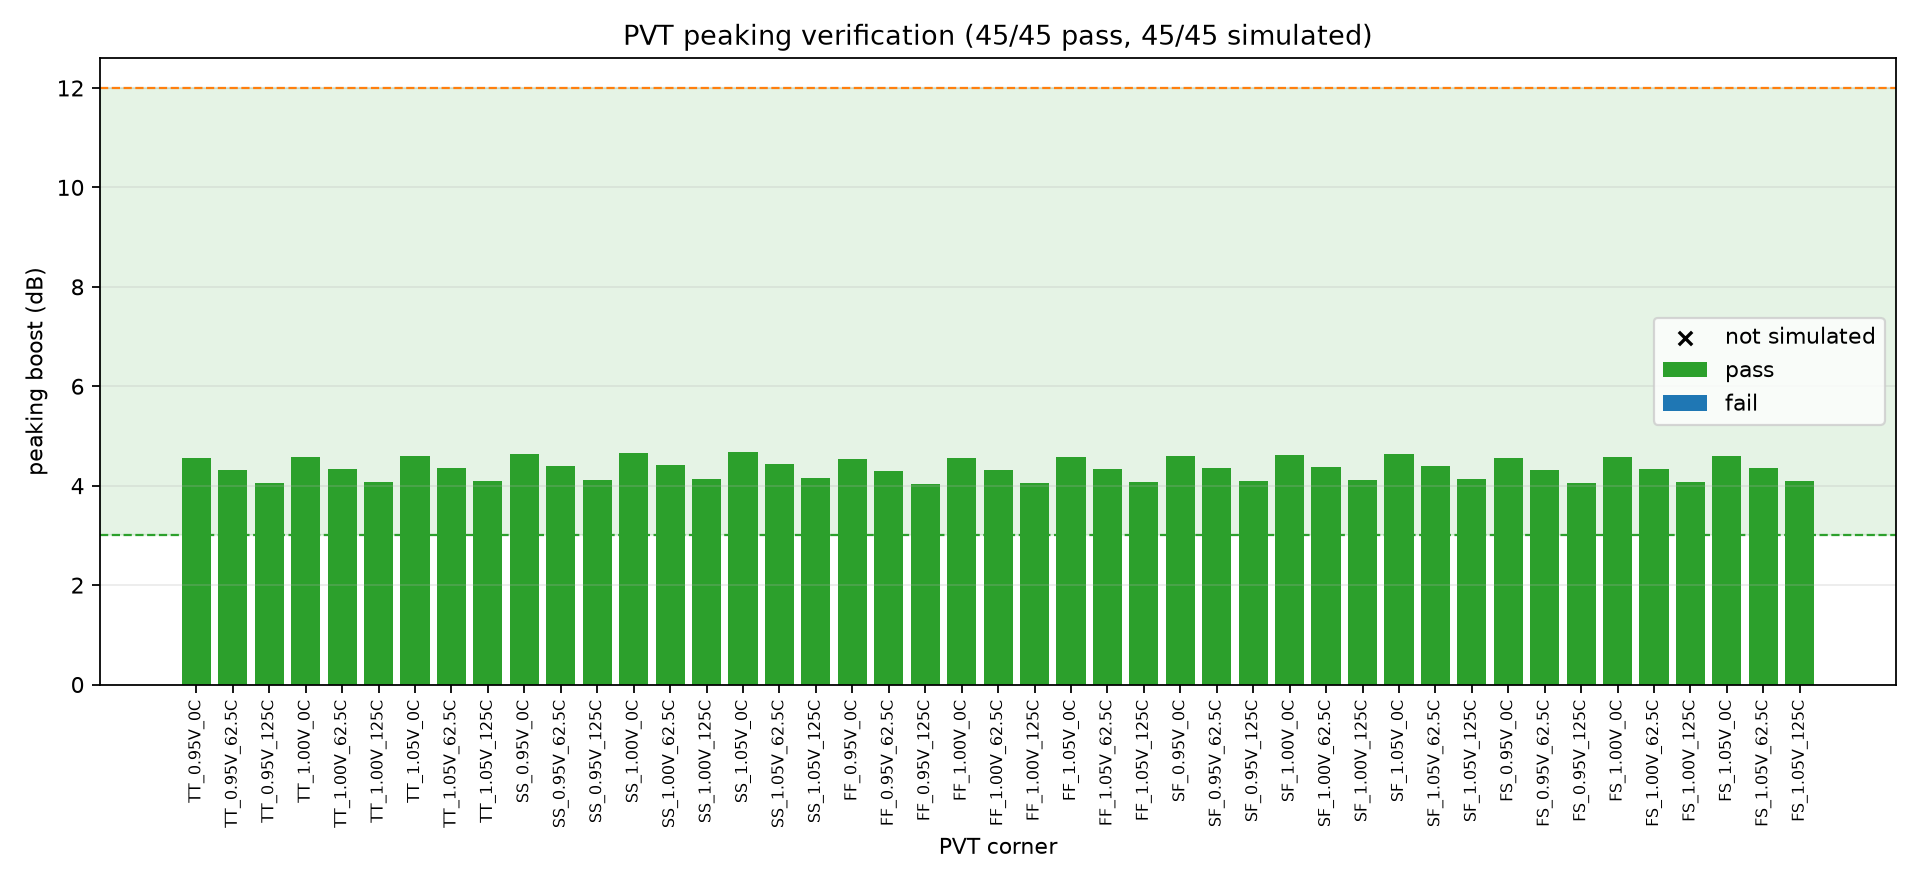
\includegraphics[width=\textwidth]{pvt_peaking}
\caption{Peaking of the curriculum policy's design across all 45 PVT corners; every corner inside the 3--12\,dB window.}
\end{minipage}
\end{figure}

\section{PVT curriculum, whole-equalizer sizing and tunability}\label{sec:curriculum}
\subsection{Curriculum across 45 corners}
Stage 1 trains at the nominal corner (TT, 1.2\,V, 27\,$^\circ$C). Stage 2 resumes the same policy with \code{--corners all --resume}: each episode is simulated at a corner drawn uniformly from the 45-corner matrix (5 process $\times$ 3 supply $\times$ 3 temperature), and the policy is not told which, so it must size for every corner from the metrics it observes. Resumed from the HD3-enforced nominal policy, the corner-randomised stage stayed at 95--96\% feasible steps from its first window (per process corner: SS 97\%, FS 96\%, FF 95\%, TT 95\%, SF 94\%), i.e.\ the nominal policy transferred and then held. In evaluation, rolled out from random designs at random corners, 24 of 24 rollouts reached a fully feasible design (19 distinct corners drawn, spanning every process, supply and temperature), median two simulation steps, worst four; the best design passes all 45 corners with HD3 at $-61.9$\,dB.

\subsection{Whole-equalizer sizing (CTLE + DFE tap)}
\code{--equalizer} extends the action to six values: the five CTLE parameters and the one-tap DFE weight in $[-0.5, 0.5]$. The DFE is applied to the CTLE's post-channel UI-centre samples whenever a waveform exists, and the post-DFE eye height drives the reward.

The first equalizer run exposed a second measurement flaw: the DFE eye was labelled by the DFE's own decisions, so a large tap separated the two decision classes by itself. The agent found this within 2k steps, drove the tap to its $+0.5$ bound and reported a 0.70\,V eye on a design whose receiver decides 54 of 127 bits wrongly. The eye is now measured against the transmitted PRBS bits (\code{rl.dfe.dfe\_eye\_against\_bits}: correlation-aligned UI-centre samples, slicer at the midpoint of the two symbol populations, DFE fed its own decisions, bit errors counted, zero eye on any error). With the honest metric a one-tap DFE still helps: the CTLE-only policy design goes from 0.327\,V to 0.455\,V at tap $+0.075$ with no errors. Trained on the corrected metric for 8k steps, the six-value policy holds 91--93\% of steps feasible with a median post-DFE eye of 0.51\,V (CTLE-only runs hold about 0.35\,V), i.e.\ it learns to spend the tap on margin. In deterministic rollouts 20 of 20 reach feasibility, median 3 steps, worst 5; the best rollout design has a raw eye of 0.325\,V that the agent's tap of $+0.062$ opens to 0.355\,V with no bit errors, at 1.36\,mW, HD3 $-71.6$\,dB and 45/45 corners.

\subsection{Tunable Nyquist frequency (1.25--2.5\,GHz)}\label{sec:tunable}
The brief asks for peaking tunable between 1.25 and 2.5\,GHz. The Nyquist frequency is a specification input (\code{--spec nyquist\_frequency\_hz=...}): it sets the frequency at which peaking is measured, the data rate and unit interval of the PRBS transient ($2\times$ Nyquist), the transient step, and the channel pole, so the channel keeps about $-10$\,dB of loss at the new Nyquist. The 2.5\,GHz policy's design peaks only 2.87\,dB at 1.25\,GHz --- it fails the spec at the lower rate --- so tunability has to be shown, not asserted. Resuming the seed-1 policy with the spec set to 1.25\,GHz (PCIe Gen 1, 2.5\,Gbps) for 3k steps: 93.5\% of steps feasible in the first 1k (the policy transfers) and 96.5\% by 3k; in evaluation 20 of 20 rollouts reach feasibility, median 2 steps, worst 5, and the best design peaks 5.23\,dB at 1.25\,GHz with a 0.350\,V / 0.94\,UI eye at 2.5\,Gbps, 1.28\,mW, HD3 $-70.9$\,dB and 45/45 corners. The retuned sizing moves the degeneration zero down in frequency ($R_s$ 365\,$\Omega$, $C_s$ 503\,fF against 182\,$\Omega$, 522\,fF at 2.5\,GHz).

\section{LLM frontend for the reward}\label{sec:llm}
\code{scripts/reward\_from\_feedback.py} turns an engineer's sentence into the reward's per-specification weights, the continuous power charge and the margin bonus (\code{rl/feedback.py}). Claude (Anthropic SDK, structured JSON output validated against a schema) produces them when credentials are present; a context-aware keyword parser is the offline fallback, so the loop never blocks on an API. The JSON is passed to \code{train\_sac.py --reward-settings} and recorded in the run's configuration; it applies from the start of that run or of a resumed curriculum stage (re-weighting a run in progress is a next step). Example, offline path:
\begin{lstlisting}
> "We are power constrained: current budget matters much more than eye margin, and we don't care about linearity"
weights: power 3.0, eye_vertical_v 0.33, hd3 0.33 (others 1.0); efficiency_weight 3.0; margin_weight 5.0
> "Open the eye as much as possible; power is not important"
weights: eye_vertical_v 3.0, power 0.33; efficiency_weight 0.33
\end{lstlisting}

\section{Deliverables and reproducibility}\label{sec:deliverables}
Every script writes JSON, CSV and PNG evidence to its output directory, and every validation writes the sized netlist \code{sized\_ctle.sp} --- the deliverable schematic --- with the device values, model source and DFE tap in its header. Prerequisites: an IHP Open PDK checkout with compiled OSDI models (\code{IHP\_PDK\_ROOT}), ngspice 44+ (\code{NGSPICE}), and \code{pip install -e .[rl]}; \code{python scripts/check\_pdk.py} confirms readiness.
\begin{lstlisting}
# train on the IHP models (nominal corner), then the corner curriculum
python scripts/train_sac.py --model-source ihp --eye-height-min 0.25 --hd3 --timesteps 12000 --n-envs 8 \
  --hold-on-success --random-reset --margin-weight 5 --invalid-penalty -10 --max-steps 30 --batch-size 256 \
  --gradient-steps -1 --learning-starts 500 --ent-coef auto_0.1 --seed 1 --output-dir reports/sac-ihp-hd3
python scripts/train_sac.py ... --corners all --resume reports/sac-ihp-hd3/sac_final.zip --timesteps 8000 \
  --output-dir reports/sac-ihp-pvt
# random-search baseline with the same reward, then evaluation and comparison
python scripts/baseline_random.py --model-source ihp --eye-height-min 0.25 --margin-weight 5 --invalid-penalty -10 \
  --evaluations 3000 --n-workers 8 --output-dir reports/baseline-ihp-3000
python scripts/evaluate_policy.py reports/sac-ihp-pvt --rollouts 24 --baseline reports/baseline-ihp-3000
# whole-equalizer sizing, CMA-ES baseline, reward weights from feedback
python scripts/train_sac.py ... --equalizer --timesteps 8000 --output-dir reports/sac-ihp-eq
python scripts/baseline_cmaes.py --model-source ihp --eye-height-min 0.25 --margin-weight 5 --invalid-penalty -10 \
  --evaluations 96 --x0 random --seed 10 --output-dir reports/cmaes-ihp-random-s10
python scripts/reward_from_feedback.py "power matters more than eye margin" --output reports/reward.json
# pre-ML pipeline evidence (100-candidate bounded search, all gates, 45 corners)
python scripts/run_validation.py --model-source ihp --output-dir reports/runs/ihp-submission
\end{lstlisting}

\begin{table}[h]\small
\begin{tabularx}{\textwidth}{l L}
\toprule
\textbf{Artifact} & \textbf{Contents}\\
\midrule
\code{reports/sac-ihp-*/} & per-step CSV, SB3 monitor files, checkpoints every 4k steps, final model, config.json, validation.json, plots, sized netlist\\
\code{reports/eval-ihp-*/} & evaluation.json (rollout statistics, per-corner breakdown, comparison), rollouts.csv, budget curve, validation plots, sized netlist\\
\code{reports/baseline-ihp-3000/}, \code{reports/cmaes-ihp-*/} & random-search and CMA-ES baselines with per-evaluation rewards and metrics; best designs validated\\
\code{reports/runs/ihp-submission-2026-09-15/} & pre-ML bounded search with every gate, regenerated on the Windows toolchain\\
\code{reports/screenshots/} & live training captures and learning curves taken every 15 minutes during training\\
\code{docs/submission\_report.md}, \code{README.md} & technical report and run instructions in the repository\\
\bottomrule
\end{tabularx}
\caption{Evidence artifacts.}
\end{table}

\section{Measurement findings}
Two measurement flaws survived the manual flow and were exposed when the agent optimised against them. Both are fixed and unit-tested, and every number in this report uses the corrected measurements.

\textbf{HD3.} The linearity gate FFT'd the last 25\,ns of a 100\,MHz tone with a rectangular window: 2.5 cycles, so the fundamental fell between 40\,MHz bins and its spectral leakage filled the 300\,MHz bin, putting a false floor of about $-25$\,dB on every design. HD3 was reported as failing in every earlier version of the evidence, and an HD3-enforced training run could not move it past $-26$\,dB because the number did not depend on the circuit (a sweep of each sizing knob over its full range confirmed this). Analysing an integer number of periods with a Hann taper gives $-58$\,dB for the same designs; the circuit was always linear enough, by about 28\,dB.

\textbf{DFE eye.} The one-tap DFE eye was labelled by the DFE's own hard decisions rather than the transmitted bits. A large tap separates the two decision classes by itself, so the metric rewards the tap regardless of the signal. The whole-equalizer agent found this within 2k steps, drove the tap to its $+0.5$ bound and reported a 0.70\,V eye on a design whose receiver decides 54 of 127 bits wrongly. The eye is now measured against the PRBS bits: correlation-aligned UI-centre samples, a slicer at the midpoint of the two symbol populations, the DFE fed its own decisions (so error propagation is modelled), bit errors counted, zero eye on any error. With the honest metric a one-tap DFE still helps: the CTLE-only policy design goes from 0.327\,V to 0.455\,V at tap $+0.075$ with no errors.

\textbf{Noise} was checked rather than corrected: the gate integrates ngspice's input-referred \code{inoise\_spectrum} over 10\,MHz--5\,GHz and reports 0.2420\,mV\,rms; ngspice's own band integral, now recorded alongside, gives 0.2417\,mV\,rms.

\section{Pre-ML pipeline evidence}
For completeness, the bounded search that preceded the RL work (\code{run\_validation.py}, 100 candidates selected on the AC gate, seed 23), regenerated on the Windows toolchain: peaking 7.527\,dB, power 0.743\,mW, eye 0.160\,V / 0.58\,UI after the channel (0.310\,V with the swept one-tap DFE, no bit errors), HD3 $-58.5$\,dB, input-referred noise 0.242\,mV\,rms, area estimate $1.09\times10^{-5}$\,mm$^2$, 45/45 PVT corners. Every gate that is unchanged since the original Linux run reproduces to all printed digits; the eye fails only because the transient gate now includes the lossy channel that the AC-only search cannot see --- the gap the RL policy closes.

\section{Deviations, limitations and next steps}
\begin{itemize}[nosep,leftmargin=*]
\item \textbf{PDK.} IHP sg13g2 instead of SkyWater sky130 (Section~\ref{sec:pdk}).
\item \textbf{DFE.} The DFE in the loop is the behavioural one-tap stage; the analog slicer in \code{DFE/} is not simulated end to end.
\item \textbf{Area} is a first-order active-device estimate, not a post-layout result.
\item \textbf{Corner awareness.} The curriculum policy is robust because it is trained blind across corners; adding the corner to the observation is a natural extension.
\item \textbf{LLM loop.} Reward weights from feedback apply at the start of a run or resumed stage, not while a run is in progress.
\item \textbf{Design space.} $R_\mathrm{load}$ sits at its 1\,k$\Omega$ bound in most designs; wider bounds and topology variants are the next lever.
\end{itemize}
Next steps, in order of value: simulate the analog DFE slicer inside the transient gate so the tap becomes a device-level knob; corner-aware observations; Bayesian-optimisation baselines at equal budget with a wall-clock comparison against a manual sweep; a closed LLM loop that reads each validation report and proposes the next reward adjustment; and, if a future round requires it, the sky130 backend.

\appendix
\section{Training configuration}
\begin{tabular}{ll}
\toprule
\textbf{Setting} & \textbf{Value}\\
\midrule
Algorithm & SAC, MlpPolicy (stable-baselines3 2.9.0, torch 2.14 CUDA)\\
Parallel environments & 8, thread-based, one ngspice process each\\
Episode & 30 steps, random initial design, held after success\\
Action scale & 0.2 of the normalised box per step\\
Reward & invalid $-10$, success $+20$, margin weight 5, power charge weight 1\\
Batch / gradient steps & 256 / one per environment step\\
Entropy coefficient & automatic, initial 0.1\\
Warm-up & 500 random steps (none when resuming)\\
Throughput & 0.5--0.7\,s per environment step on a 12-core laptop; 12k steps in about 2\,h\\
Tests & 59, run without ngspice\\
\bottomrule
\end{tabular}

\section{Sized netlist of the curriculum policy's best design (excerpt)}
\begin{lstlisting}
* AutoAnalog-RL sized CTLE
* model source: ihp_ngspice
* W_in = 2.01908e-05
* R_load = 1000
* I_bias = 0.000930072
* R_s = 260.642
* C_s = 3.2956e-13
* Parameterized differential gm-C CTLE.
.param VDD=1.2
VDD vdd 0 1.2
Vinp txP 0 DC 0.6 AC 1
... (full file: reports/eval-ihp-pvt/sized_ctle.sp)
\end{lstlisting}

\end{document}
